%%%%%%%%%%%%%%%%%%%%%%%%%%%%%%%%%%%%%%%%%	
% a0poster Portrait Poster
% LaTeX Template
% Version 1.0 (22/06/13)
%
% The a0poster class was created by:
% Gerlinde Kettl and Matthias Weiser (tex@kettl.de)
% 
% This template has been downloaded from:
% http://www.LaTeXTemplates.com
%
% License:
% CC BY-NC-SA 3.0 (http://creativecommons.org/licenses/by-nc-sa/3.0/)
%
%%%%%%%%%%%%%%%%%%%%%%%%%%%%%%%%%%%%%%%%%

%----------------------------------------------------------------------------------------
%	PACKAGES AND OTHER DOCUMENT CONFIGURATIONS
%----------------------------------------------------------------------------------------

\documentclass[a0,landscape]{a0poster}

\usepackage[margin=2in]{geometry}

%\usepackage{multicol} % This is so we can have multiple columns of text side-by-side
%\columnsep=100pt % This is the amount of white space between the columns in the poster
%\columnseprule=3pt % This is the thickness of the black line between the columns in the poster

\usepackage[svgnames]{xcolor} % Specify colors by their 'svgnames', for a full list of all colors available see here: http://www.latextemplates.com/svgnames-colors

\usepackage{times} % Use the times font
%\usepackage{palatino} % Unco\emph{}mment to use the Palatino font

\usepackage{graphicx} % Required for including images
\graphicspath{{figures/}} % Location of the graphics files
\usepackage{booktabs} % Top and bottom rules for table
\usepackage[font=normalsize,labelfont=bf]{caption} % Required for specifying captions to tables and figures
\usepackage{amsfonts, amsmath, amsthm, amssymb} % For math fonts, symbols and environments
\usepackage{wrapfig} % Allows wrapping text around tables and figures

%\usepackage{apacite}
%\renewcommand\bibliographytypesize{\small}

\usepackage{flowfram}


\newstaticframe{\textwidth}{0.2\paperheight}{0pt}{0.8\textheight}[head]

\newflowframe{0.29\paperwidth}{0.85\textheight}
{0.0\paperwidth}{-0.05\paperheight}[leftcolumn]

\newflowframe{0.30\textwidth}{0.49\textheight}
{0.35\paperwidth}{0.30\paperheight}[centercolumn]

\newflowframe{0.30\textwidth}{0.49\textheight}
{0.67\paperwidth}{0.30\paperheight}[rightcolumn]

\newstaticframe{0.67\paperwidth}{0.20\paperheight}
{0.37\paperwidth}{0pt}[statico]

\begin{document}

%----------------------------------------------------------------------------------------
%	POSTER HEADER 
%----------------------------------------------------------------------------------------

% The header is divided into two boxes:
% The first is 75% wide and houses the title, subtitle, names, university/organization and contact information
% The second is 25% wide and houses a logo for your university/organization or a photo of you
% The widths of these boxes can be easily edited to accommodate your content as you see fit

%\begin{minipage}[b]{0.60\linewidth}
%\veryHuge \color{NavyBlue} \textbf{Personality and Blood Chemistry Associations with Cardiovascular Health in Chimpanzees} \color{Black}\\ % Title
%\huge \textbf{Drew M Altschul\textsuperscript{1}, David Sinn\textsuperscript{2}, \& Alexander Weiss\textsuperscript{1}}\\[0.5cm] % Author(s)
%\huge \textsuperscript{1}The University of Edinburgh\\[0.4cm] % University/organization
%\huge \textsuperscript{2}University of Texas\\[0.4cm]
%%\huge \textsuperscript{2}Columbia University\\[0.4cm] % University/organization
%\Large \texttt{d.m.altschul@sms.ed.ac.uk}\\
%\end{minipage}
%%
%\begin{minipage}[b]{0.40\linewidth}
%
\includegraphics[width=26cm]{EdiU.jpg}\\
%%\bigskip{}
%\end{minipage}

\begin{staticcontents*}{head}

\begin{tabular}{p{0.51\linewidth} p{0.20\linewidth}}
    \vspace{0pt} 
    \linespread{0.9}
\veryHuge \color{NavyBlue} \textbf{Personality and Blood Chemistry Associations with Cardiovascular Health in Chimpanzees} \color{Black}\\ % Title
\huge \textbf{Drew M Altschul\textsuperscript{1}, David Sinn\textsuperscript{2}, \& Alexander Weiss\textsuperscript{1}}\\[0.5cm] % Author(s)
\huge \textsuperscript{1}The University of Edinburgh\\[0.4cm] % University/organization
\huge \textsuperscript{2}University of Texas\\[0.4cm]
%\huge \textsuperscript{2}Columbia University\\[0.4cm] % University/organization
\Large \texttt{d.m.altschul@sms.ed.ac.uk}\\
\linespread{1.0}
    & 
    \vspace{-25ex}
    \hspace{30cm}
    
\includegraphics[width=26cm]{EdiU.jpg}\\
   
\end{tabular}
\end{staticcontents*}

%\vspace{1cm} % A bit of extra whitespace between the header and poster content

%----------------------------------------------------------------------------------------

%\begin{multicols}{3} % This is how many columns your poster will be broken into, a portrait poster is generally split into 2 columns
\hyphenchar\font=-1

%----------------------------------------------------------------------------------------
%	ABSTRACT
%----------------------------------------------------------------------------------------

%\color{DarkSlateGrey} % Navy color for the abstract
%
%\begin{abstract}
%
%Sed fringilla tempus hendrerit. Vestibulum ante ipsum primis in faucibus orci luctus et ultrices posuere cubilia Curae; Etiam ut elit sit amet metus lobortis consequat sit amet in libero. Lorem ipsum dolor sit amet, consectetur adipiscing elit. Phasellus vel sem magna. Nunc at convallis urna. isus ante. Pellentesque condimentum dui. Etiam sagittis purus non tellus tempor volutpat. Donec et dui non massa tristique adipiscing. Quisque vestibulum eros eu. Phasellus imperdiet, tortor vitae congue bibendum, felis enim sagittis lorem, et volutpat ante orci sagittis mi. Morbi rutrum laoreet semper. Morbi accumsan enim nec tortor consectetur non commodo nisi sollicitudin. Proin sollicitudin. Pellentesque eget orci eros. Fusce ultricies, tellus et pellentesque fringilla, ante massa luctus libero, quis tristique purus urna nec nibh.
%
%\end{abstract}

%----------------------------------------------------------------------------------------
%	INTRODUCTION
%----------------------------------------------------------------------------------------

\color{Black} % SaddleBrown color for the introduction

\section*{Introduction}

Metabolic syndrome is directly related to the onset of diabetes and heart disease, while being indirectly associated with a multitude of other conditions, such as depression \cite{shively2002depression}. A wide array of chimpanzee personality models have been developed and linked to other psychological capacities, such as intelligence and subjective well-being \cite{weiss2002subjective}. Moreover, personality has been shown to be related to physical traits  \cite{wilson2014personality} and specific genes \cite{latzman2014personality}.

%Heart disease and diabetes are complex conditions, poorly understood in humans as well as other primates. 
Since associations have been found between many aspects of human personality and cardiovascular risk factors and biomarkers \cite{sutin2010cholesterol}, might we find similar relationships in chimpanzees? Controlling for environmental variables in humans will always be difficult; less so with captive chimps. We therefore analyzed associations between personality, blood biomarkers, and physical characteristics like BMI and blood pressure in chimpanzees.

%In a group of personality related chimps, we analyzed blood biomarkers in conjunction with physical characteristics like BMI and blood pressure, to see how chimpanzee personality relates to cardiovascular and metabolic physiology.


%----------------------------------------------------------------------------------------
%	OBJECTIVES
%----------------------------------------------------------------------------------------

\color{NavyBlue}
\section*{Main Questions}

\begin{itemize}
\item Are relationships between metabolic syndrome symptoms and personality, as seen in humans, to be found in chimpanzees?
\item How do blood biomarkers associate with known risk factors?
\item Can we uncover the causal relationships between risk factors, symptoms, and biomarkers?
\end{itemize}

%----------------------------------------------------------------------------------------
%	MATERIALS AND METHODS
%----------------------------------------------------------------------------------------

\color{Maroon}
\section*{Materials and Methods}

\begin{itemize}
\item 196 chimpanzees were assessed 
\item Personality ratings were gathered using the 43-item Chimpanzee Personality Questionnaire
\item Hematological biomarkers analyzed were triglycerides, glucose, total cholesterol, and lymphocytes, gathered across multiple time points during regular check-ups
\item Physical characteristics controlled for were BMI, age, and sex
\item Associations were tested with linear mixed-effect models
\end{itemize}
%for a combination of personality, via the 43-item Chimpanzee , and hematological biomarkers and physical characteristics, gathered across multiple time points during regular check-ups. Associations between biomarkers and other characteristics were tested with linear mixed-effect models, controlling for age, sex, and BMI. The only random effect was introduced around the individual subjects.

%----------------------------------------------------------------------------------------
%	RESULTS 
%----------------------------------------------------------------------------------------

\color{Black}
\section*{Results}

All confidence intervals are at 95\%. Significant positive associations were found between Openness ($\beta$=3.96, C.I.:[1.80, 6.12]) and blood pressure, as well as Extraversion ($\beta$=-7.76, C.I.:[-11.5, -4.02]) and blood pressure.

We also wanted to see if personality impacted physiology, so directly tested for associations between personality and blood biomarker levels. Though we observed some marginal effects from other biomarkers, triglycerides showed the strongest relationships, with Agreeableness ($\beta$=-24.1, C.I.:[-36.3, -11.9]) and Openness ($\beta$=10.64, C.I.:[1.51, 19.7]).

 %triglyceride levels, which have been implicated in the development of heart disease and metabolic syndrome \cite{sutin2010cholesterol}. Mixed modeling revealed non-significant trends between triglyceride levels and Extraversion and Openness, and a significant, very strong relationship with Agreeableness ($\beta$=-24.138877, S.E.= 6.710). 

%Agreeableness, associated with human ``Type A'' personalities, has a mixed history of being associated with cardiovascular health \cite{sutin2010cholesterol}. Type A personalities clearly relates to cardiovascular disease at some level, but it remains unclear whether the effect is behavioral, physiological, or even genetic. Elucidating the specific impacts of personality on a cardiovascular health requires a more nuanced analytic approach.

%
%\begin{wraptable}{l}{12cm} % Left or right alignment is specified in the first bracket, the width of the table is in the second
%\begin{tabular}{l l l}
%\toprule
%\textbf{Treatments} & \textbf{Response 1} & \textbf{Response 2}\\
%\midrule
%Treatment 1 & 0.0003262 & 0.562 \\
%Treatment 2 & 0.0015681 & 0.910 \\
%Treatment 3 & 0.0009271 & 0.296 \\
%\bottomrule
%\end{tabular}
%\captionof{table}{\color{Green} Table caption}
%\end{wraptable}
%


%----------------------------------------------------------------------------------------
%	CONCLUSIONS
%----------------------------------------------------------------------------------------

\color{NavyBlue}
\section*{Summary}

\begin{itemize}
\color{NavyBlue}
\item A biochemical system like that sampled from the chimpanzee (and human) blood stream offers us a window onto the function and dysfunction of an array of other systems.
\item Insight from a chimpanzee personality perspective suggests that Extraversion, Openness to experience, and Agreeableness are related to cardiovascular disease symptoms.
%\color{NavyBlue}
\item These results match up well with human data, contributing to a more robust understanding of general primate cardiovascular health.
\item Agreeableness, associated with human ``Type A'' personalities, has a mixed history of being associated with cardiovascular health \cite{sutin2010cholesterol}.
\item Type A personality clearly relates to cardiovascular disease at some level, but it remains unclear whether the effect is behavioral, physiological, or even genetic.
\item Chimpanzee and human metabolic health appear quite similar. Results from both species, applied with comparative perspective, stand to improve the health of humans and captive chimps, but a more nuanced analysis of these data is called for.


\end{itemize}


%----------------------------------------------------------------------------------------
%	FUTURE
%----------------------------------------------------------------------------------------

\color{Maroon}
\section*{Where to go from here}

\begin{itemize}
\item Complex physiological pathways are not easily described by linear regression.
\item In order to grapple with the causal impacts of our variables on one another, we will use structural equation modeling to evaluate which relationships between personality, biomarkers, and physical manifestations are meaningful. A hypothetical model is shown in Figure 1.
\item Additional data ought to be gathered from more primate species, and more path models ought to be tested so we can understand what symptoms and biomarkers are the best indicators of current and future health.

\end{itemize}	




 %----------------------------------------------------------------------------------------
%	REFERENCES
%----------------------------------------------------------------------------------------

\color{Black}
{\footnotesize
\nocite{*} % Print all references regardless of whether they were cited in the poster or not
\bibliographystyle{plain} % Plain referencing style
\bibliography{apabibl}
}

%%----------------------------------------------------------------------------------------
%%	ACKNOWLEDGEMENTS
%%----------------------------------------------------------------------------------------
%
%\section*{Acknowledgements}
%
%Etiam fermentum, arcu ut gravida fringilla, dolor arcu laoreet justo, ut imperdiet urna arcu a arcu. Donec nec ante a dui tempus consectetur. Cras nisi turpis, dapibus sit amet mattis sed, laoreet.
%
%%----------------------------------------------------------------------------------------

%\end{multicols}


%----------
%Figure placed at bottom
%----------
%\begin{minipage}[b]{1\linewidth}

\begin{staticcontents*}{statico}

%\vspace{0.5cm}
% figure environment won't work here
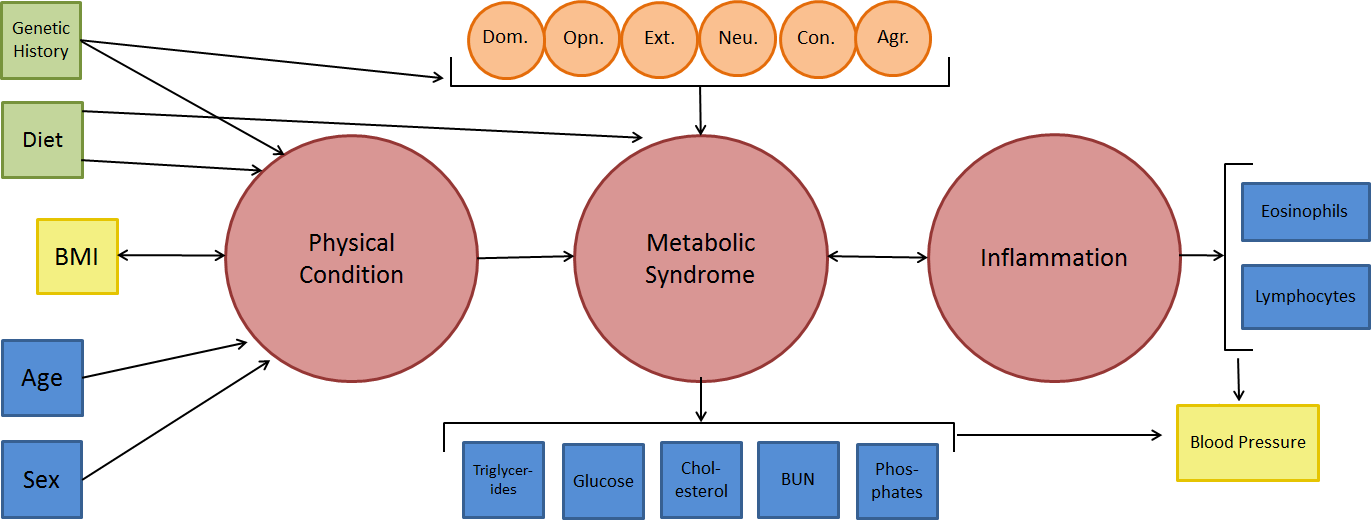
\includegraphics[width=0.85\textwidth]{2PassFig.png}
\hspace{-1cm}
\captionof{figure}{\color{DarkSlateGrey} Proposed model of relationships among chimpanzee personality, blood biomarkers, and physical characteristics.}

\end{staticcontents*}

%\end{minpage}


\end{document}